
\label{sec:metodologia}

Este capítulo describe el procedimiento: qué se hizo en cada etapa, con qué insumos, con qué regla de decisión y con qué sustento. Las ecuaciones están en el Marco teórico (Sección~\ref{sec:marco-teorico}) y aquí solo se citan; los resultados de cada etapa están en la Sección~\ref{sec:resultados}, que tiene los mismos títulos en el mismo orden. La Figura~\ref{fig:met_flujo} muestra las 16 etapas, agrupadas en cuatro fases: la preparación de los datos (etapas 1 a 4), la construcción de la respuesta y de las covariables (5 a 8), el modelo Fay-Herriot clásico que sirve de benchmark no espacial (9 a 12), y el modelo espacial con la estimación en los municipios (13 a 16).

\begin{figure}[!htbp]
\centering
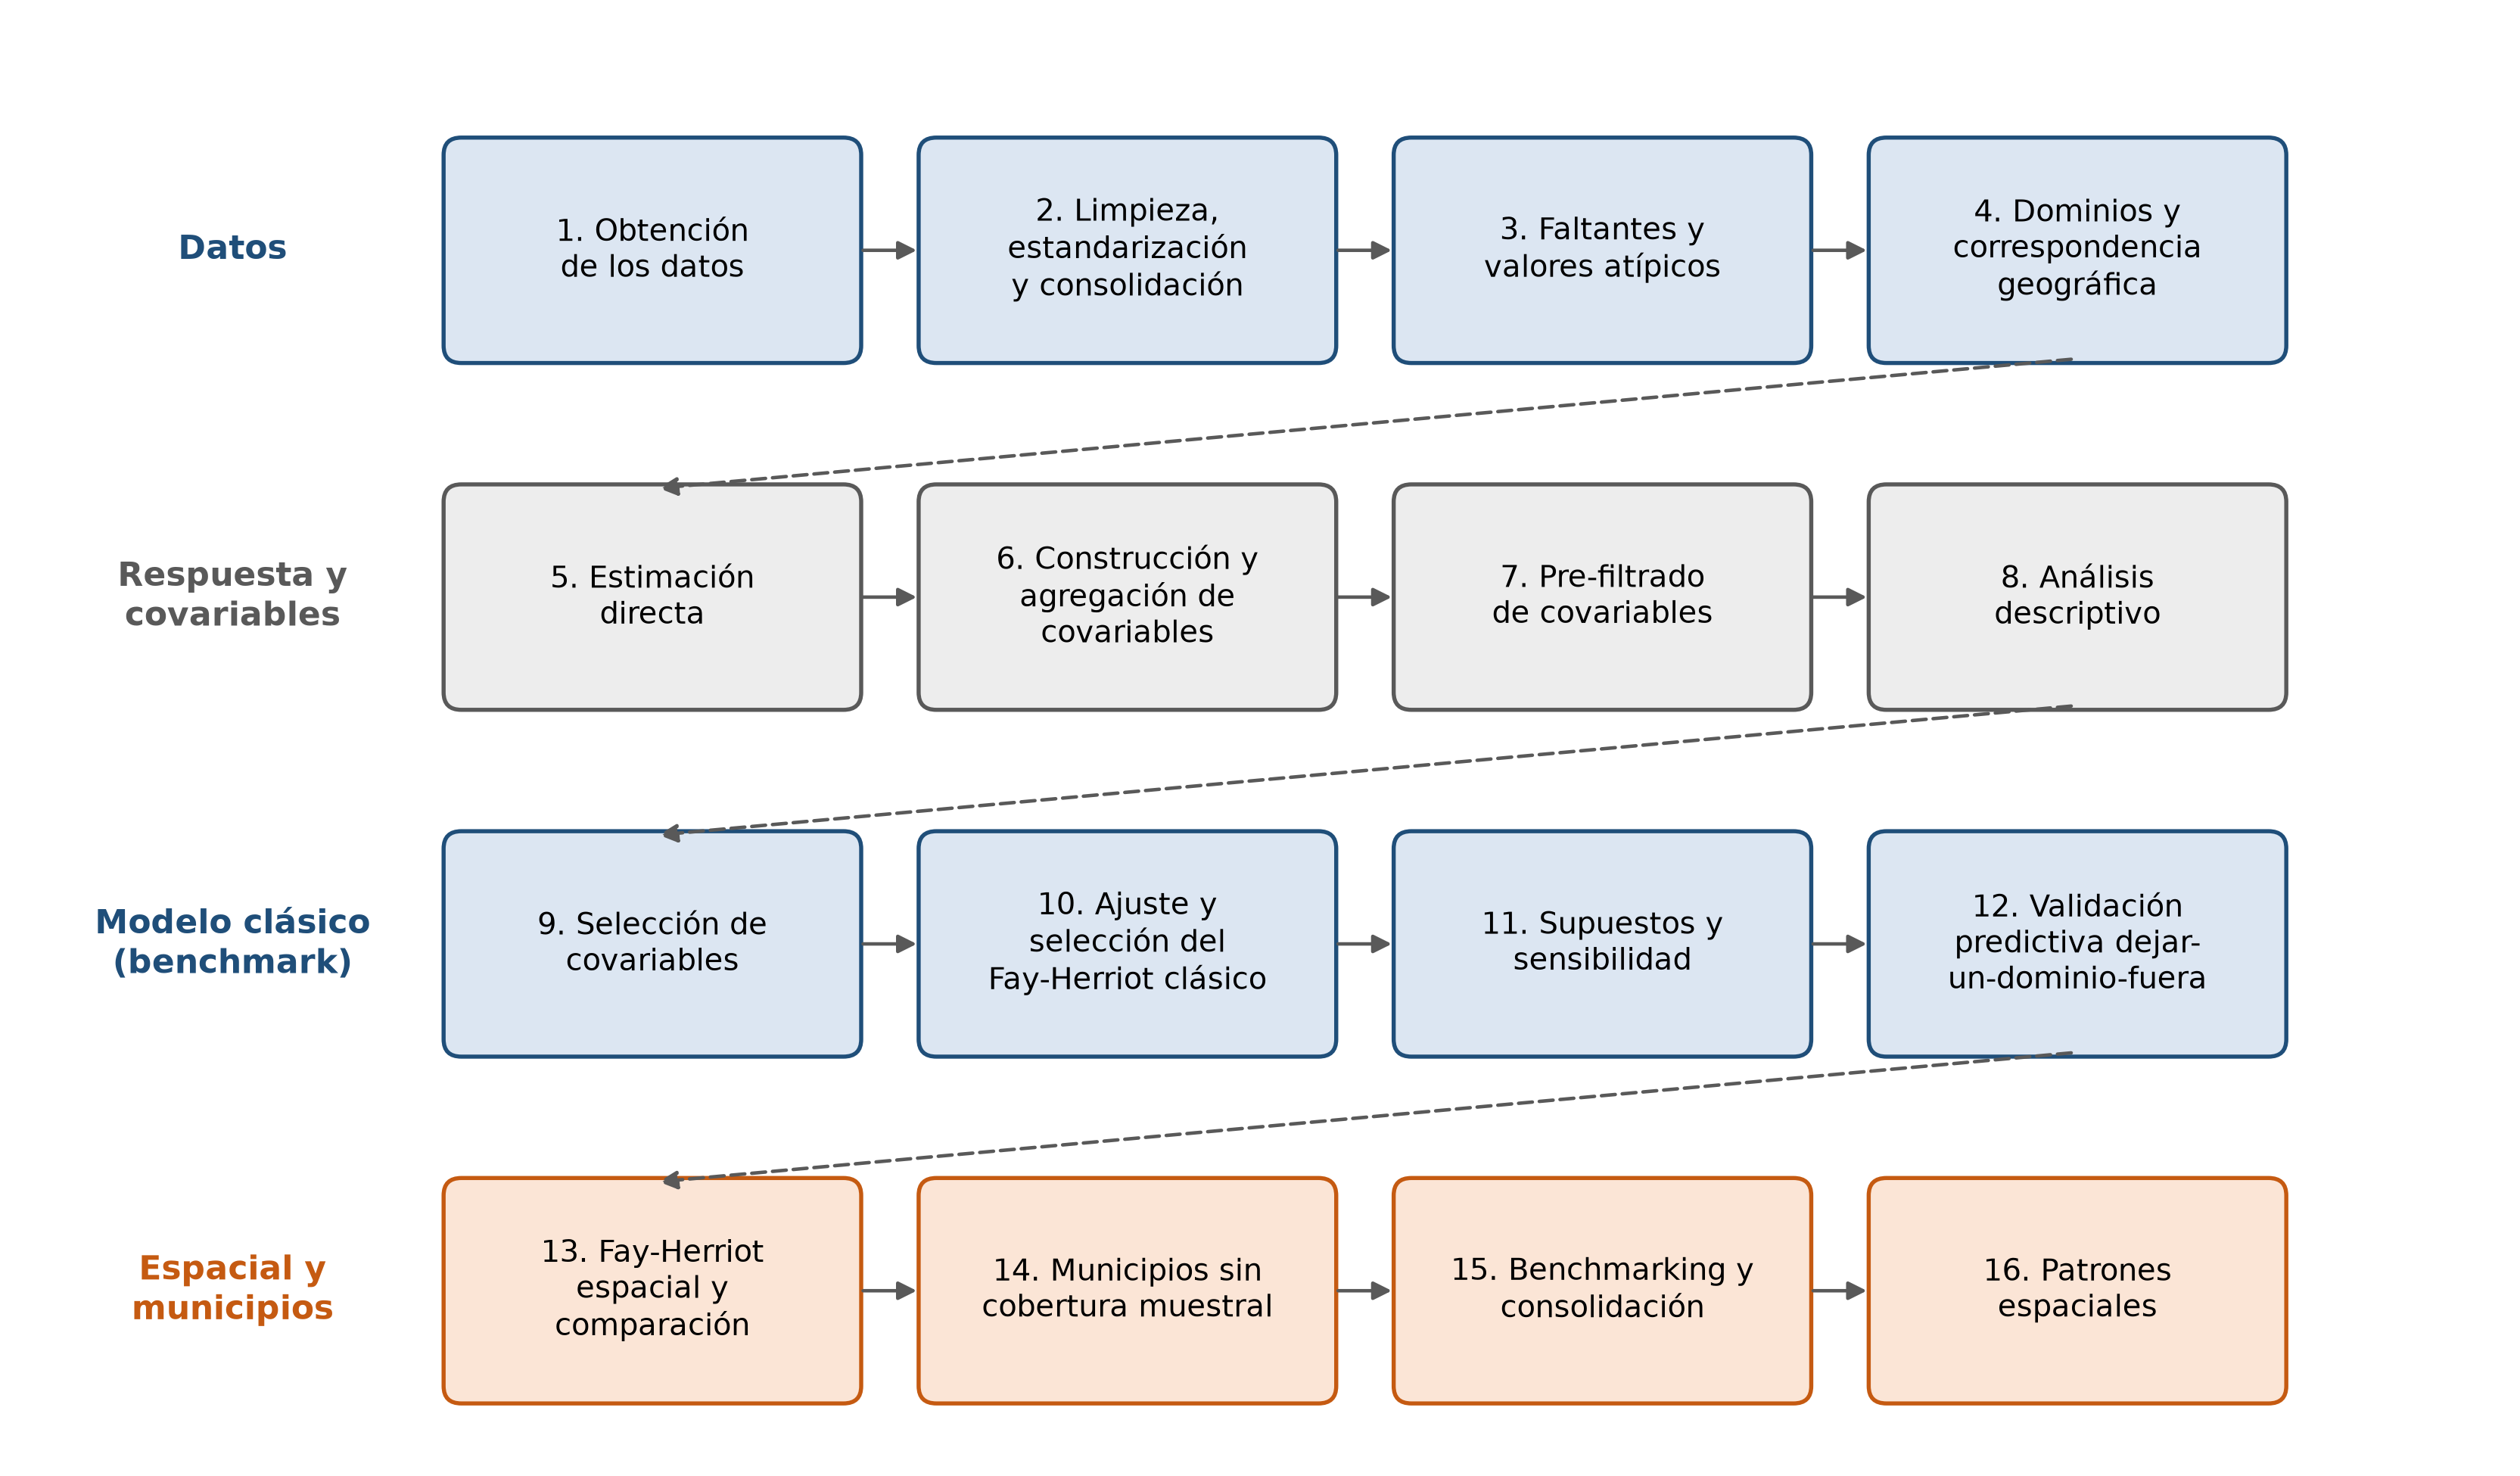
\includegraphics[width=\linewidth]{img/met_flujo_general.png}
\caption{Etapas de la metodología. Las flechas continuas unen etapas de una misma fase y las discontinuas el paso de una fase a la siguiente. Cada etapa tiene una sección con el mismo número en este capítulo y en Resultados.}
\label{fig:met_flujo}
\end{figure}

Cada etapa se presenta con una ficha que reúne sus entradas, las transformaciones, la regla de decisión, los parámetros fijados de antemano, el sustento y la salida. Todo el procesamiento corrió en Databricks, con tablas en un catálogo de Unity Catalog organizado en capas, y se despliega como un conjunto de trabajos programados que repiten la cadena completa; el linaje de tablas y la forma de reproducir cada etapa están en el Apéndice~\ref{app:reproducibilidad}.

%--------------------------------------------------------------------------------------
\section{Obtención de los datos}
\label{sec:met_obtencion}

Las cuatro fuentes de la Sección~\ref{sec:datos} se cargaron sin modificar su contenido, siguiendo una arquitectura de medallón: una capa bronce con los datos como llegan, una capa plata con los datos limpios y consolidados, y una capa oro con la tabla analítica de mercado laboral (Tabla~\ref{tab:met_obtencion}). La capa bronce permite repetir cualquier transformación posterior sin volver a descargar las fuentes.

\begin{table}[!htbp]
\centering
\small
\caption{Ficha de la etapa 1: obtención de los datos.}
\label{tab:met_obtencion}
\renewcommand{\arraystretch}{1.15}
\begin{tabularx}{\linewidth}{>{\raggedright\arraybackslash}p{2.8cm} >{\raggedright\arraybackslash}X}
\toprule
Elemento & Contenido \\
\midrule
Entradas & Archivos de texto de la GEIH 2018 por mes, módulo y sección (cabecera y resto); archivo de factores de expansión recalculados con el CNPV 2018; archivos de TerriData en formato largo; DIVIPOLA; hojas del anexo del DANE \\
Transformaciones & Lectura de cada archivo por separado y unión por nombre de columna; columna con el archivo de origen de cada registro; ningún valor se modifica \\
Regla de decisión & Se cargan solo los módulos necesarios para la condición de actividad (Tabla~\ref{tab:dimensiones-geih-modulos}) \\
Sustento & Definiciones de la encuesta \cite[p.~20]{DANE_GEIH_Metodologia2016} \\
Salida & Capa bronce: una tabla por módulo y sección de la GEIH, una para TerriData y una por hoja del anexo \\
\bottomrule
\end{tabularx}
\end{table}

%--------------------------------------------------------------------------------------
\section{Limpieza, estandarización y consolidación}
\label{sec:met_limpieza}

La GEIH reparte la información de una persona en varios módulos, y en el marco antiguo cada módulo en dos archivos. Esta etapa los une en una tabla con una fila por persona y verifica que la clasificación resultante sea coherente (Tabla~\ref{tab:met_limpieza}). La llave de una persona es la concatenación del período, la vivienda, el hogar y el orden dentro del hogar; la vivienda (período y directorio) se conserva aparte porque es la unidad del bootstrap de la etapa 5.

Dos correcciones de esta etapa cambian las cifras y por eso se describen. Primero, los archivos de enero a marzo de 2018 traen las columnas en otro orden; leerlos todos a la vez asignaba los valores por posición, corría las columnas y dejaba a toda la población en edad de trabajar como activa. Se leyó cada archivo por separado y se unieron por nombre de columna. Segundo, en el marco antiguo el factor de expansión sale solo del archivo recalculado con el CNPV 2018; si una persona queda sin factor o con factor no positivo, el procesamiento se detiene antes de escribir la tabla, en lugar de asignarle cero.

\begin{table}[!htbp]
\centering
\small
\caption{Ficha de la etapa 2: limpieza, estandarización y consolidación.}
\label{tab:met_limpieza}
\renewcommand{\arraystretch}{1.15}
\begin{tabularx}{\linewidth}{>{\raggedright\arraybackslash}p{2.8cm} >{\raggedright\arraybackslash}X}
\toprule
Elemento & Contenido \\
\midrule
Entradas & Capa bronce de la GEIH (identificadores de texto, indicadores binarios de condición, edad entera, factor de expansión continuo) \\
Transformaciones & Nombres de columna y tipos comunes a ambos marcos; separador decimal; unión de cabecera y resto; PEA del marco antiguo como la PET que no figura entre los inactivos; unión de los módulos a características generales por la llave de persona; factor de expansión por marco; código de municipio del área y nombre del departamento desde las tablas de dimensión \\
Regla de decisión & El procesamiento se detiene si alguna persona queda sin factor de expansión o con factor no positivo \\
Verificaciones & Porcentaje de llaves de cada módulo sin pareja en características generales; identidades PEA = OC + DS y PET = PEA + PEI (Ecuación~\ref{eq:identidades}) por año, mes y dominio, con la cuenta de los casos que las rompen; personas sin factor \\
Sustento & Factores CNPV 2018 y salto de serie al mezclar factores \cite[pp.~3, 19]{DANE_GEIH_Series2022} \\
Salida & Tabla de mercado laboral (capa oro) y tablas de reconciliación \\
\bottomrule
\end{tabularx}
\end{table}

En TerriData la limpieza normalizó los nombres de departamento y entidad (mayúsculas y sin tildes), unificó el valor numérico y el cualitativo en un solo campo, clasificó cada indicador como numérico si al menos el 95~\% de sus registros es numérico, y pasó la base a formato ancho, con una fila por entidad, año y mes y una columna por indicador. Cuatro comprobaciones (número de filas antes y después, duplicados de la llave, una muestra aleatoria comparada en ambos formatos y el total de valores no nulos) se imprimen como aprobadas o no, sin detener el proceso.

%--------------------------------------------------------------------------------------
\section{Tratamiento de datos faltantes y valores atípicos}
\label{sec:met_faltantes}

La Tabla~\ref{tab:met_faltantes} reúne qué se hizo con los faltantes y los atípicos según el papel de cada variable. No se imputó ningún valor: los indicadores de condición de actividad se construyen por la pertenencia a un módulo, el factor de expansión faltante detiene el procesamiento y una covariable incompleta queda fuera del modelo. Tampoco se eliminaron dominios ni municipios por ser atípicos: con 23 dominios, cada uno es un territorio real, y su influencia se mide con la distancia de Cook y con el reajuste sin cada dominio (etapa 11).

\begin{table}[!htbp]
\centering
\small
\caption{Ficha de la etapa 3: tratamiento de datos faltantes y valores atípicos.}
\label{tab:met_faltantes}
\renewcommand{\arraystretch}{1.15}
\begin{tabularx}{\linewidth}{>{\raggedright\arraybackslash}p{3.2cm} >{\raggedright\arraybackslash}X}
\toprule
Variable o caso & Tratamiento \\
\midrule
Condición de actividad (PET, PEA, OC, DS, PEI) & Es 1 si la persona está en el módulo que la define y 0 si no; la ausencia en el módulo de ocupados, por ejemplo, significa que no está ocupada \\
Factor de expansión & Sin imputación: si falta o no es positivo, el procesamiento se detiene (etapa 2) \\
Registros sin código de área & No se usan: no pertenecen a ninguno de los 23 dominios (Sección~\ref{sec:datos_geih}) \\
Covariable con faltantes en los dominios & Sale en el pre-filtrado (etapa 7) \\
Covariable con faltantes en los municipios objetivo & No entra al catálogo activo: sin ella no hay estimación sintética (etapa 6) \\
Valores no interpretables en TerriData & Se convierten a nulo y siguen la regla anterior \\
Valores atípicos & No se eliminan ni se recortan; se señalan con la regla del diagrama de caja (Ecuación~\ref{eq:iqr}) y su influencia se mide en la etapa 11 \\
\bottomrule
\end{tabularx}
\end{table}

Algunos criterios habituales no aplican. No hay covariables categóricas ni codificación de variables indicadoras: las 18 candidatas son cuantitativas. No hay una búsqueda de hiperparámetros: los parámetros del procedimiento (umbrales, réplicas, semillas) se fijaron antes de ver los resultados, y en el modelo espacial se comparan cuatro matrices de proximidad como escenarios, no como valores para optimizar.

%--------------------------------------------------------------------------------------
\section{Definición de los dominios de estimación y correspondencia geográfica}
\label{sec:met_dominios}

El dominio de estimación es la unidad que identifica la GEIH: la ciudad capital o la ciudad con su área metropolitana. Así, la tasa directa de Cali es la de Cali A.M., la misma unidad para la que publica el DANE. Cada dominio lleva el código DIVIPOLA de su capital, y una tabla de dimensión enumera sus municipios miembro con la composición de la metodología de la encuesta (Tabla~\ref{tab:met_dominios}). Una tabla de auditoría documenta, para cada dominio, el período, el código de área de la GEIH, el nombre con que lo publica el DANE, la geografía de la tasa (las cabeceras) y la de las covariables (el municipio completo), los municipios miembro con su código, la regla de agregación de las covariables y la tasa directa frente a la del DANE en la misma ventana.

\begin{table}[!htbp]
\centering
\small
\caption{Ficha de la etapa 4: definición de los dominios y correspondencia geográfica.}
\label{tab:met_dominios}
\renewcommand{\arraystretch}{1.15}
\begin{tabularx}{\linewidth}{>{\raggedright\arraybackslash}p{2.8cm} >{\raggedright\arraybackslash}X}
\toprule
Elemento & Contenido \\
\midrule
Entradas & Código de área de la GEIH; DIVIPOLA; lista de capitales y de municipios de cada área metropolitana \\
Transformaciones & Código de área $\to$ código del departamento de la capital $\to$ código DIVIPOLA de la capital; una fila por municipio miembro con el dominio al que pertenece y su tipo (ciudad o ciudad con A.M.) \\
Regla de decisión & Membresía estricta de la GEIH; los registros sin código de área no se usan \\
Sustento & Composición de las áreas metropolitanas \cite[p.~9]{DANE_GEIH_Metodologia2016} \\
Salida & Tabla de dominios (32 capitales, 52 municipios miembro; 23 dominios con muestra en 2018) y tabla de auditoría de los 23 dominios \\
\bottomrule
\end{tabularx}
\end{table}

%--------------------------------------------------------------------------------------
\section{Estimación directa de la tasa de desempleo}
\label{sec:met_directa}

La respuesta del modelo es la tasa directa de cada dominio en el año 2018, con la varianza que el modelo trata como conocida (Tabla~\ref{tab:met_directa}). La ventana de un año calendario se eligió frente al mes y al trimestre porque reúne más viviendas por dominio, lo que reduce la varianza de la estimación; la sensibilidad de la tasa a las tres ventanas se calculó aparte con el mismo estimador y no alimenta el modelo. El DANE no publica la tasa anual por ciudad, así que la cifra de referencia de cada dominio se reconstruye como la suma de desocupados sobre la suma de la PEA de los cuatro trimestres del año que no se superponen.

\begin{table}[!htbp]
\centering
\small
\caption{Ficha de la etapa 5: estimación directa.}
\label{tab:met_directa}
\renewcommand{\arraystretch}{1.15}
\begin{tabularx}{\linewidth}{>{\raggedright\arraybackslash}p{2.8cm} >{\raggedright\arraybackslash}X}
\toprule
Elemento & Contenido \\
\midrule
Entradas & Tabla de mercado laboral: indicador de desocupado (binario), factor de expansión (continuo), vivienda; personas de 15 años y más de la PEA en los 12 meses de 2018; tabla de dominios \\
Transformaciones & Estimador de Hájek por dominio (Ecuación~\ref{eq:hajek}); bootstrap por viviendas con el dominio como estrato (Ecuaciones~\ref{eq:var_bootstrap} y~\ref{eq:ic_bootstrap}); varianza de Taylor con las mismas viviendas (Ecuación~\ref{eq:taylor}); CV (Ecuación~\ref{eq:cve}); PEA expandida media mensual, peso del benchmarking \\
Regla de decisión & Clase del CV: confiable ($<5~\%$), aceptable ($5$ a $<20~\%$), no confiable ($\geq 20~\%$) \\
Parámetros & Ventana de 12 meses con cierre en diciembre (alternativa admitida: trimestre); $B = \num{2000}$ réplicas; semilla 42; edad mínima 15 años \\
Verificaciones & Tasa de cada dominio y tasa conjunta ponderada por la PEA frente a las del DANE en la misma ventana; bootstrap frente a Taylor \\
Sustento & \cite[pp.~21--22, 26--27, 61]{morales2021smallarea}; \cite[pp.~12, 15]{DANE_GEIH_Metodologia2016}; umbral del 20~\%: \cite[pp.~14--15]{Molina2019} \\
Salida & Por dominio: tasa, error estándar bootstrap, intervalo del 95~\%, CV y clase, error estándar de Taylor, personas, desocupados y viviendas de la muestra, PEA expandida \\
\bottomrule
\end{tabularx}
\end{table}

El bootstrap no reproduce el estrato interno ni el segmento, que no vienen en los microdatos. Por eso no se afirma que la varianza obtenida quede por encima ni por debajo de la del diseño, y la etapa 11 evalúa qué pasa con el modelo si se reemplaza.

%--------------------------------------------------------------------------------------
\section{Construcción y agregación de las covariables}
\label{sec:met_covariables}

Las covariables candidatas salen de un catálogo construido con la revisión de literatura del proyecto: entra un indicador solo si un estudio lo relaciona con el desempleo, y cada entrada declara el signo esperado de esa relación y su referencia, antes de calcular ninguna cifra (Tabla~\ref{tab:met_covariables}). La exigencia de una relación interpretable sigue la recomendación de que las variables auxiliares tengan una explicación acorde con la disciplina que estudia el fenómeno \cite[p.~453]{morales2021smallarea}. Las justificaciones del catálogo hablan de asociación, no de causa. El catálogo completo, con el código de TerriData y la referencia de cada entrada, está en el Apéndice~\ref{app:catalogo}.

\begin{table}[!htbp]
\centering
\small
\caption{Ficha de la etapa 6: construcción y agregación de las covariables.}
\label{tab:met_covariables}
\renewcommand{\arraystretch}{1.15}
\begin{tabularx}{\linewidth}{>{\raggedright\arraybackslash}p{2.8cm} >{\raggedright\arraybackslash}X}
\toprule
Elemento & Contenido \\
\midrule
Entradas & TerriData en formato ancho (indicadores cuantitativos: porcentajes, tasas, valores per cápita, puntajes); tabla de dominios; tasas directas \\
Transformaciones & Valor del dominio por razón de totales con el denominador propio de cada indicador (Ecuación~\ref{eq:agregacion}; denominadores en la Tabla~\ref{tab:covariables_datos}); unión con las tasas por dominio, año y mes; tabla de municipios objetivo con sus covariables a nivel municipal y, para Cali y Yumbo, el dominio al que pertenecen \\
Regla de decisión & Entrada activa si tiene referencia, dato para 2018 y valor en todos los municipios objetivo; toda covariable debe tener una regla de agregación, y el valor de un dominio es nulo si le falta a alguno de sus miembros \\
Parámetros & Departamentos objetivo: 19 (Cauca) y 76 (Valle del Cauca) \\
Verificaciones & Sensibilidad de las covariables de las 7 áreas metropolitanas a ponderar todas por la población de 15 años y más en lugar de su denominador propio; el procesamiento se detiene si a un miembro le falta un peso, si falta un miembro de un dominio con A.M. entre los objetivos o si no queda ningún municipio objetivo \\
Sustento & Valor del área \cite[p.~425]{morales2021smallarea}; razón de totales \cite[p.~21]{morales2021smallarea} \\
Salida & Catálogo (18 activas y 6 sin dato utilizable, con su motivo); tabla de 23 dominios con respuesta y covariables; tabla de 83 municipios objetivo \\
\bottomrule
\end{tabularx}
\end{table}

El índice de incidencia del conflicto armado, que estaba en una versión anterior del catálogo, se retiró: mide el conflicto en el propio municipio y no la llegada de población desplazada que motivaba su inclusión, toma 13 valores distintos por redondeo y tiene una correlación de 0.92 con la tasa de homicidios. No se sustituyó por otro indicador. La tasa de tránsito a la educación superior se conservó por decisión del equipo.

%--------------------------------------------------------------------------------------
\section{Pre-filtrado de covariables}
\label{sec:met_prefiltrado}

El pre-filtrado retira las candidatas que no se pueden usar, sin mirar su relación con la tasa de desempleo (Tabla~\ref{tab:met_prefiltrado}). Por eso no se repite dentro de la validación predictiva de la etapa 12.

\begin{table}[!htbp]
\centering
\small
\caption{Ficha de la etapa 7: pre-filtrado de covariables.}
\label{tab:met_prefiltrado}
\renewcommand{\arraystretch}{1.15}
\begin{tabularx}{\linewidth}{>{\raggedright\arraybackslash}p{2.8cm} >{\raggedright\arraybackslash}X}
\toprule
Elemento & Contenido \\
\midrule
Entradas & Tabla de 23 dominios con todas las columnas de TerriData del período \\
Transformaciones & Conversión numérica tolerante a errores de las columnas de texto \\
Regla de decisión & Completitud: sin faltantes en los 23 dominios. Variabilidad: CV descriptivo (Ecuación~\ref{eq:cv_descriptivo}) $\geq 0.001$ y proporción de dominios con el valor modal $\leq 0.90$. Sin filtro por correlación con la respuesta \\
Parámetros & CV mínimo 0.001; proporción modal máxima 0.90; los pares con $|r| \geq 0.999$ se reportan como duplicados, sin decidir \\
Verificaciones & Cascada (candidatas que pasan cada filtro) y sensibilidad del número de sobrevivientes a los dos umbrales de variabilidad \\
Sustento & Una columna constante es colineal con el intercepto y deja singular la matriz de la Ecuación~\ref{eq:gls}; los dos criterios no dependen de la unidad del indicador \\
Salida & Covariables pre-filtradas, cascada y sensibilidad \\
\bottomrule
\end{tabularx}
\end{table}

%--------------------------------------------------------------------------------------
\section{Análisis descriptivo}
\label{sec:met_descriptivo}

El análisis descriptivo caracteriza la tasa directa, su precisión y las candidatas activas, en tres niveles (Tabla~\ref{tab:met_descriptivo}). No decide: una variable asimétrica no se descarta por serlo y un dominio extremo no se retira. No se aplicó análisis de componentes principales, porque sus combinaciones no tienen una lectura territorial y exigen decidir cuántas retener. Tampoco se aplicó la prueba de Shapiro-Wilk a las covariables: el modelo supone normalidad de los efectos y de los errores, no de las covariables.

\begin{table}[!htbp]
\centering
\small
\caption{Ficha de la etapa 8: análisis descriptivo.}
\label{tab:met_descriptivo}
\renewcommand{\arraystretch}{1.15}
\begin{tabularx}{\linewidth}{>{\raggedright\arraybackslash}p{2.8cm} >{\raggedright\arraybackslash}X}
\toprule
Elemento & Contenido \\
\midrule
Entradas & Tasa directa, su error estándar y $\psi_d$; 18 candidatas activas; diccionario de indicadores \\
Univariado & Posición, dispersión, asimetría y CV descriptivo (Ecuación~\ref{eq:cv_descriptivo}); valores señalados por la regla del diagrama de caja (Ecuación~\ref{eq:iqr}) con el dominio al que corresponden; diagramas de caja en escala estandarizada (solo gráfica) \\
Bivariado & Pearson y Spearman con la tasa (Ecuaciones~\ref{eq:pearson} y~\ref{eq:spearman}) e intervalo de Fisher (Ecuación~\ref{eq:ic_fisher}); diagramas de dispersión \\
Multivariado & Matriz de correlaciones reordenada por agrupamiento de enlace promedio con la distancia de la Ecuación~\ref{eq:distancia_correlacion}; pares con $|r| > 0.80$ \\
Regla de decisión & Ninguna: la etapa es descriptiva \\
Salida & Tablas univariada y bivariada; figuras de la respuesta, de su distribución por dominio, de las candidatas y de sus correlaciones; interpretación calculada desde los datos \\
\bottomrule
\end{tabularx}
\end{table}

%--------------------------------------------------------------------------------------
\section{Selección de covariables}
\label{sec:met_seleccion}

La selección elige las covariables del modelo en cinco pasos (Tabla~\ref{tab:met_seleccion}). Cada paso se puede verificar por separado, y el recorrido de cada candidata queda registrado. Decide el modelo Fay-Herriot univariado con las mismas $\psi_d$ del modelo final, no la correlación de Pearson, porque el primero pondera cada dominio por la precisión de su estimación directa.

\begin{table}[!htbp]
\centering
\small
\caption{Ficha de la etapa 9: selección de covariables.}
\label{tab:met_seleccion}
\renewcommand{\arraystretch}{1.15}
\begin{tabularx}{\linewidth}{>{\raggedright\arraybackslash}p{2.8cm} >{\raggedright\arraybackslash}X}
\toprule
Paso & Contenido \\
\midrule
1. Asociación & Fay-Herriot univariado por candidata (REML y GLS), con intervalo de Wald de $\beta_1$, valor $p$ y correlación ponderada $r_w$ (Ecuación~\ref{eq:r_ponderada}), que ordena y fija el signo; valor $q$ de Benjamini-Hochberg sobre las 18 (Ecuación~\ref{eq:bh}). Forma funcional como diagnóstico: término cuadrático y logaritmo frente a lineal por AIC \\
2. Robustez y soporte & Diagnósticos, no filtros: Cook (Ecuación~\ref{eq:cook}) y cambio de $r_w$ al retirar cada dominio (dependencia si Cook $> 4/n$ y el cambio supera 0.10 o invierte el signo); proporción de municipios objetivo dentro del rango de los dominios, con advertencia por debajo de 0.80 \\
3. Redundancia & Grupos por enlace completo con $|r| \geq 0.80$ entre todos sus pares; representante: el primer integrante elegible con menor Cook máximo; si no es elegible, se pasa al siguiente \\
4. Ficha de decisión & Elegible si $q \leq 0.10$; el signo esperado se compara con el observado como diagnóstico; se seleccionan las $\lfloor n/10 \rfloor$ elegibles de mayor $|r_w|$ (Ecuación~\ref{eq:pmax}); si no hay elegibles, el conjunto queda vacío y el modelo usa solo el intercepto \\
5. Verificación & VIF del conjunto (Ecuación~\ref{eq:vif}); si una supera 5, se reemplaza por la siguiente elegible; residuos parciales; repetición de la selección exigiendo el signo esperado, como sensibilidad \\
Parámetros & $q \leq 0.10$; $|r| \geq 0.80$; 10 observaciones por parámetro; VIF $\leq 5$; Cook $4/n$ y cambio 0.10 (inspección); soporte 0.80 (advertencia) \\
Sustento & \cite[pp.~453--454]{morales2021smallarea}; \cite{BenjaminiHochberg1995}; VIF: \cite[sec.~9.4]{MontgomeryPeckVining2012}; cota, 0.80 y $4/n$: convenciones del trabajo \\
Salida & Diagnósticos por candidata, grupos de redundancia, ficha de decisión, verificación, trazabilidad y conjunto seleccionado \\
\bottomrule
\end{tabularx}
\end{table}

En una versión anterior, la robustez descartaba candidatas. Se cambió a diagnóstico porque la regla $4/n$ sirve para inspeccionar observaciones, no para excluir variables, y porque el umbral de 0.10 en el cambio de la correlación queda por debajo del error de muestreo de $r$ con 23 dominios; la literatura de referencia no usa la influencia para seleccionar \cite[pp.~453--454]{morales2021smallarea}. No se hizo una búsqueda exhaustiva de especificaciones por AIC entre las 18 candidatas: con 23 dominios produciría muchas especificaciones equivalentes y reutilizaría los mismos datos que ajustan el modelo.

%--------------------------------------------------------------------------------------
\section{Ajuste y selección del modelo Fay-Herriot clásico (benchmark)}
\label{sec:met_fh_clasico}

Con el conjunto seleccionado se ajustan varias especificaciones candidatas del modelo base Fay-Herriot clásico y se elige una, que es el benchmark no espacial contra el que se compara el modelo espacial (Tabla~\ref{tab:met_fh_clasico}). Las especificaciones se nombran EC1 (el conjunto seleccionado), EC2, EC3 y siguientes (sus subconjuntos no vacíos) y EC0 (solo intercepto). No son los modelos finales del objetivo específico 1: son las variantes entre las que se elige el benchmark.

\begin{table}[!htbp]
\centering
\small
\caption{Ficha de la etapa 10: ajuste y selección del Fay-Herriot clásico.}
\label{tab:met_fh_clasico}
\renewcommand{\arraystretch}{1.15}
\begin{tabularx}{\linewidth}{>{\raggedright\arraybackslash}p{2.8cm} >{\raggedright\arraybackslash}X}
\toprule
Elemento & Contenido \\
\midrule
Entradas & Tasa directa $\hat{\theta}_d$ y $\psi_d$ de los 23 dominios; covariables seleccionadas \\
Transformaciones & Para cada especificación: $\hat{\sigma}_u^2$ por REML, $\hat{\boldsymbol{\beta}}$ por GLS (Ecuación~\ref{eq:gls}), EBLUP (Ecuación~\ref{eq:eblup_a}), ECM de Prasad-Rao (Ecuaciones~\ref{eq:ecm_eblup} y~\ref{eq:ecm_componentes}), CV, AIC y AICc con la verosimilitud ML (Ecuaciones~\ref{eq:loglik} y~\ref{eq:aic}); error de estimación dejar-un-dominio-fuera de cada especificación, como descripción \\
Regla de decisión & Compiten las especificaciones con todas sus covariables con $p < 0.05$ (EC0 cumple de forma trivial); entre ellas, la de menor AIC, y entre las que difieren en $\Delta\text{AIC} \leq 2$, la de menos covariables. Si ninguna con covariables cumple, compiten todas y la elección se reporta como excepción \\
Parámetros & $\alpha = 0.05$; $\Delta\text{AIC} \leq 2$; aviso si $\max_d \hat{\gamma}_d < 0.01$ ($\hat{\sigma}_u^2 \approx 0$) o si alguna tasa cae fuera de $[0, 100]$ \\
Sustento & \cite[pp.~427, 434--441, 453--454]{morales2021smallarea}; AICc: \cite{HurvichTsai1989}; $\Delta\text{AIC} \leq 2$: convención \\
Salida & Diagnósticos y coeficientes de cada especificación; tabla de selección con el criterio aplicado; EBLUP, ECM, CV y $\hat{\gamma}_d$ de los 23 dominios con el benchmark \\
\bottomrule
\end{tabularx}
\end{table}

Los valores $p$ de esta etapa son descriptivos. Los mismos 23 dominios filtran las candidatas, las seleccionan y estiman los coeficientes, así que los coeficientes son asociaciones condicionales a la selección y no se interpretan como efectos causales. La literatura de referencia no trata este punto; el trabajo lo reporta como una limitación y lo examina en las etapas 11 y 12. El ECM y la distancia de Cook no intervienen en la elección: se reportan para el benchmark.

%--------------------------------------------------------------------------------------
\section{Validación de supuestos y sensibilidad del benchmark}
\label{sec:met_supuestos}

Esta etapa revisa los supuestos del benchmark y mide cuánto cambian sus coeficientes y sus estimaciones cuando cambian los datos o la varianza de muestreo (Tabla~\ref{tab:met_supuestos}). Ninguno de estos análisis cambia el modelo elegido ni las tasas publicadas.

\begin{table}[!htbp]
\centering
\small
\caption{Ficha de la etapa 11: validación de supuestos y sensibilidad del benchmark.}
\label{tab:met_supuestos}
\renewcommand{\arraystretch}{1.15}
\begin{tabularx}{\linewidth}{>{\raggedright\arraybackslash}p{2.8cm} >{\raggedright\arraybackslash}X}
\toprule
Análisis & Contenido \\
\midrule
Normalidad & Residuos estandarizados (Ecuación~\ref{eq:residuos}): media (cercana a cero por construcción), desviación, histograma y Shapiro-Wilk (Ecuación~\ref{eq:shapiro}), leído como «sin evidencia fuerte en contra», no como prueba de normalidad \\
Influencia & Distancia de Cook (Ecuación~\ref{eq:cook}) con $\hat{\sigma}_u^2$ fijo; reajuste sin el dominio más influyente \\
Estabilidad de coeficientes & 23 reajustes dejando un dominio fuera (reestimando $\hat{\sigma}_u^2$): mínimo y máximo de cada $\hat{\beta}_j$, dominio que los produce, cambio estandarizado (Ecuación~\ref{eq:dfbeta}), cambios de signo y de significancia; efecto en los EBLUP de los otros dominios, en las estimaciones de los 83 municipios y en su clase de confiabilidad. Bootstrap de dominios con la especificación fija \\
Varianza de muestreo & Varianzas alternativas: bootstrap por personas, Taylor, GVF A y B (Ecuación~\ref{eq:gvf}); nueve escenarios del modelo: base, Taylor, GVF A y $\psi_d \times k$; en cada uno se reajustan todas las especificaciones y se vuelve a elegir con la misma regla; se comparan $\hat{\sigma}_u^2/\bar{\psi}$, $\hat{\gamma}_d$, $\hat{\boldsymbol{\beta}}$, EBLUP, CV, clase, $\lambda_1$ y estimaciones municipales \\
Parámetros & Umbrales de influencia: 1 error estándar y 0.5 puntos porcentuales; \num{1000} réplicas bootstrap, semilla 42; $k \in \{1/3, 1/2, 2/3, 3/2, 2, 3\}$ \\
Sustento & \cite{ShapiroWilk1965, Cook1977}; GVF: \cite[p.~427]{morales2021smallarea}, \cite[pp.~15--16]{MarinTralmaGuerrero2024}, \cite[p.~15]{Tellez2020}; $\hat{\sigma}_u^2/\bar{\psi}$: \cite[p.~143]{Benedetti2024}; umbrales de influencia: convención \\
Salida & Tablas de estabilidad, de influencia por dominio y de escenarios de varianza; mapa de calor de la influencia \\
\bottomrule
\end{tabularx}
\end{table}

%--------------------------------------------------------------------------------------
\section{Validación predictiva dejar-un-dominio-fuera}
\label{sec:met_validacion}

Las cifras del ajuste con los 23 dominios no dicen qué tan bien estima el modelo un lugar sin encuesta, porque el EBLUP de un dominio se apoya en su propia estimación directa. La validación predictiva dejar-un-dominio-fuera imita ese uso: retira un dominio, ajusta con los otros 22 y lo estima como si no tuviera encuesta (Tabla~\ref{tab:met_validacion}). Se hace de dos formas. Con las covariables del benchmark fijas, solo se reestiman $\hat{\boldsymbol{\beta}}$ y $\hat{\sigma}_u^2$; es optimista, porque esas covariables se eligieron viendo al dominio retirado. Con el procedimiento completo, en cada iteración se repiten la selección de la etapa 9 y la elección de la etapa 10 con los 22 dominios que quedan. La diferencia entre ambos errores es el costo de haber seleccionado con los mismos datos.

\begin{table}[!htbp]
\centering
\small
\caption{Ficha de la etapa 12: validación predictiva dejar-un-dominio-fuera.}
\label{tab:met_validacion}
\renewcommand{\arraystretch}{1.15}
\begin{tabularx}{\linewidth}{>{\raggedright\arraybackslash}p{2.8cm} >{\raggedright\arraybackslash}X}
\toprule
Elemento & Contenido \\
\midrule
Entradas & 23 dominios con respuesta, $\psi_d$ y las 18 candidatas pre-filtradas; benchmark de la etapa 10 \\
Transformaciones & Para cada dominio: ajuste sin él y estimación sintética $\mathbf{x}_d^\top\hat{\boldsymbol{\beta}}_{(-d)}$ con tres especificaciones: covariables fijas, procedimiento completo y solo intercepto (referencia) \\
Métricas & RMSE, MAE, sesgo, RMSE corregida por ruido, $Z_\psi$, $Z_{\text{pred}}$ (media, desviación y cobertura) y habilidad frente al modelo de solo intercepto (Ecuación~\ref{eq:metricas_val}); error dentro de muestra para medir el optimismo; conjunto elegido en cada iteración y frecuencia de cada covariable \\
Regla de decisión & Ninguna: la validación no cambia el benchmark. Si el procedimiento completo estima peor que el modelo de solo intercepto (habilidad negativa), se reporta como limitación, con la inestabilidad del conjunto entre iteraciones \\
Verificaciones & Con los 23 dominios, la selección y la elección deben reproducir el conjunto y el benchmark; si no, se advierte y se sigue \\
Parámetros & Cobertura nominal del 95~\% \\
Sustento & Análisis propio; lectura del estimador fuera de muestra: \cite[p.~441]{morales2021smallarea}, \cite[p.~144]{Benedetti2024} \\
Salida & Errores por dominio y ejercicio, métricas por ejercicio, selección por iteración y frecuencia de selección \\
\bottomrule
\end{tabularx}
\end{table}

Con 23 dominios las métricas resultan de 23 estimaciones y se leen como orden de magnitud.

%--------------------------------------------------------------------------------------
\section{Modelo Fay-Herriot espacial y comparación con el benchmark}
\label{sec:met_espacial}

El objetivo específico 1 compara el benchmark con especificaciones espaciales. La comparación es controlada: misma respuesta, mismas $\psi_d$, mismos 23 dominios y las mismas covariables del benchmark, sin volver a seleccionarlas. Cambia solo la estructura de los efectos de área (Ecuación~\ref{eq:sar}). La Tabla~\ref{tab:met_espacial} es la ficha de la etapa y la Tabla~\ref{tab:met_comparacion}, el contenido de la comparación.

\begin{table}[!htbp]
\centering
\small
\caption{Ficha de la etapa 13: modelo Fay-Herriot espacial y comparación con el benchmark.}
\label{tab:met_espacial}
\renewcommand{\arraystretch}{1.15}
\begin{tabularx}{\linewidth}{>{\raggedright\arraybackslash}p{2.8cm} >{\raggedright\arraybackslash}X}
\toprule
Elemento & Contenido \\
\midrule
Entradas & Las mismas del benchmark, más las coordenadas de las cabeceras de los 23 dominios y de los 83 municipios objetivo \\
Matriz de proximidad & Distancia de gran círculo entre cabeceras; cada dominio con A.M. es un solo nodo, ubicado en su capital; cuatro escenarios: 3 y 5 vecinos más cercanos, distancia inversa con potencia 1 y 2; estandarización por filas \\
Estructuras & «Muestra»: solo los 23 dominios. «Completa»: dominios y municipios objetivo, con verosimilitud marginal de los dominios. Ocho especificaciones en total \\
Estimación & $\hat{\sigma}_u^2$ y $\hat{\rho}$ por REML; AIC con ML; LRT de $\rho = 0$ (Ecuación~\ref{eq:lrt}); perfil de verosimilitud de $\rho$; SEBLUP (Ecuación~\ref{eq:seblup}); ECM por bootstrap paramétrico \\
Regla de decisión & Escenario de referencia: menor AIC entre las estructuras «completa» con $|\hat{\rho}| < 0.99$. El espacial se prefiere al clásico solo si $p(\text{LRT}) < 0.05$ en la estructura «muestra» del mismo escenario. El $\Delta$AIC y la validación se reportan, no deciden \\
Parámetros & $k \in \{3, 5\}$; potencias $\{1, 2\}$; $|\rho| \leq 0.99$; 500 réplicas bootstrap, semilla 42; \num{9999} permutaciones para Moran; $\alpha = 0.05$ \\
Sensibilidades & Ubicación del nodo de un A.M. en la media de sus municipios en lugar de la capital; $\hat{\rho}$ de la estructura «completa» con distintos conjuntos de municipios objetivo \\
Sustento & \cite[pp.~490--494]{morales2021smallarea}; \cite[pp.~146--149]{Benedetti2024}; \cite{PetrucciSalvati2006, PratesiSalvati2008}; escenarios de la matriz: convención \\
Salida & Comparación de especificaciones, cuadro comparativo, Moran, perfil de $\rho$, validación, coeficientes y sensibilidades \\
\bottomrule
\end{tabularx}
\end{table}

La vecindad se define por distancia y no por contigüidad porque los 23 dominios son ciudades dispersas y los municipios objetivo no limitan con ellas. El valor de $k$ y la potencia no los identifican los datos: $k = 3$ es la conexión mínima con la que ninguna ciudad queda aislada; con $k > 5$ y 23 nodos la matriz deja de ser local; la potencia 1 decae despacio y la 2 concentra el peso en las ciudades cercanas. Por eso se reportan los cuatro escenarios. El $\hat{\rho}$ de la estructura «completa» depende de qué municipios sin dato se incluyen como nodos, por lo que su signo no se interpreta y la prueba de $\rho = 0$ se hace en la estructura «muestra».

\begin{table}[!htbp]
\centering
\small
\caption{Contenido de la comparación entre el benchmark y el modelo espacial. Las diferencias se reportan sin pruebas adicionales al LRT de $\rho = 0$: con 23 dominios se describen, no se prueban.}
\label{tab:met_comparacion}
\renewcommand{\arraystretch}{1.15}
\begin{tabularx}{\linewidth}{>{\raggedright\arraybackslash}p{2.6cm} >{\raggedright\arraybackslash}X >{\raggedright\arraybackslash}p{2.6cm}}
\toprule
Elemento & Qué se compara & Ecuaciones \\
\midrule
Ajuste & $\hat{\sigma}_u^2$, $\hat{\rho}$, AIC, $\Delta$AIC y LRT del benchmark y de las ocho especificaciones espaciales & \ref{eq:aic}, \ref{eq:lrt} \\
Residuos & I de Moran de los residuos del clásico y del SEBLUP con la misma matriz y la misma estandarización; mapa de residuos & \ref{eq:moran} \\
Fuera de muestra & Validación dejar-un-dominio-fuera con covariables fijas para el sintético clásico, el sintético espacial y el espacial con efecto, con las métricas de la etapa 12 & \ref{eq:metricas_val} \\
Incertidumbre & ECM y CV del EBLUP y del SEBLUP en los 23 dominios; peso de la directa $\hat{\gamma}_d$ y $\hat{\gamma}^{S}_d$; ECM y CV de las estimaciones de los 83 municipios & \ref{eq:ecm_eblup}, \ref{eq:gamma_esp}, \ref{eq:var_sintetica} \\
Estimaciones & Diferencia en puntos porcentuales entre ambas estimaciones en dominios y municipios: media, máximo absoluto, correlación de Pearson y de Spearman; municipios que cambian de clase de confiabilidad & \ref{eq:pearson}, \ref{eq:spearman}, \ref{eq:cve} \\
Coeficientes & $\hat{\beta}_j$ y su error estándar en ambos modelos, y la diferencia medida en errores estándar del clásico & \ref{eq:gls} \\
\bottomrule
\end{tabularx}
\end{table}

Aparte de la comparación controlada, se reporta la comparación entre el benchmark, elegido con la regla de la etapa 10, y la especificación espacial de referencia, elegida con la regla de esta etapa entre los cuatro escenarios de la matriz.

%--------------------------------------------------------------------------------------
\section{Estimación en los municipios sin cobertura muestral}
\label{sec:met_sin_muestra}

Los 83 municipios objetivo reciben la estimación del modelo con sus propias covariables (Tabla~\ref{tab:met_sin_muestra}). En el clásico es el predictor sintético (Ecuación~\ref{eq:sintetico}); en el espacial, el predictor espacial (Ecuación~\ref{eq:pred_espacial}), que agrega el efecto que el modelo asigna a cada municipio a partir de los residuos de los dominios cercanos. Cali y Yumbo no son nodos de la matriz: forman parte del dominio Cali A.M. y reciben la parte sintética con sus propias covariables más el efecto estimado de su dominio. Cada estimación se acompaña de su estado de extrapolación y de una calidad reportada que no se reduce al CV.

\begin{table}[!htbp]
\centering
\small
\caption{Ficha de la etapa 14: estimación en los municipios sin cobertura muestral.}
\label{tab:met_sin_muestra}
\renewcommand{\arraystretch}{1.15}
\begin{tabularx}{\linewidth}{>{\raggedright\arraybackslash}p{2.8cm} >{\raggedright\arraybackslash}X}
\toprule
Elemento & Contenido \\
\midrule
Entradas & Covariables de los 83 municipios; $\hat{\boldsymbol{\beta}}$, $\widehat{\operatorname{Cov}}(\hat{\boldsymbol{\beta}})$ y $\hat{\sigma}_u^2$ del benchmark; ajuste espacial del escenario de referencia \\
Transformaciones & Predictor sintético y su ECM (Ecuaciones~\ref{eq:sintetico} y~\ref{eq:var_sintetica}); predictor espacial con ECM por bootstrap (nodos) o sintético (Cali y Yumbo); rango de cada covariable en los dominios y estado de extrapolación (Ecuación~\ref{eq:hnew}); estimación con covariables recortadas al rango y aporte extrapolado; reajuste sin cada dominio y amplitud de la estimación de cada municipio \\
Regla de decisión & Estado: fuera del rango, combinación atípica o dentro del rango. Calidad reportada: clase de CV, más «condicional al modelo» en todo municipio, más «extrapolado (fuera del rango)» o «extrapolado (combinación atípica)» si corresponde. La estimación publicada no cambia por la extrapolación \\
Sustento & \cite[pp.~3, 441--442, 453]{morales2021smallarea}; \cite[pp.~38--39]{Molina2019}; \cite[p.~144]{Benedetti2024}; \cite[sec.~3.8]{MontgomeryPeckVining2012} \\
Salida & Estimación de cada municipio con ambos modelos, ECM, CV, estado, covariable que más aporta a la extrapolación, aporte extrapolado, rangos y sensibilidad \\
\bottomrule
\end{tabularx}
\end{table}

%--------------------------------------------------------------------------------------
\section{Benchmarking y consolidación de las estimaciones}
\label{sec:met_benchmarking}

El benchmarking hace que las estimaciones del modelo reproduzcan cifras directas confiables de un territorio mayor, en dos niveles (Tabla~\ref{tab:met_benchmarking}). El resto de los municipios conserva la estimación sintética sin ajustar: el departamento tiene estimación directa anual en la GEIH, pero se calcula con los registros sin código de área, que este trabajo no usa; un tercer nivel departamental queda como extensión posible.

\begin{table}[!htbp]
\centering
\small
\caption{Ficha de la etapa 15: benchmarking y consolidación.}
\label{tab:met_benchmarking}
\renewcommand{\arraystretch}{1.15}
\begin{tabularx}{\linewidth}{>{\raggedright\arraybackslash}p{2.8cm} >{\raggedright\arraybackslash}X}
\toprule
Elemento & Contenido \\
\midrule
Entradas & EBLUP y ECM de los 23 dominios; PEA expandida de cada dominio; tasa directa del conjunto de los 23 dominios y cifra del DANE de la misma ventana; estimaciones de Cali y Yumbo y su población de 15 años y más \\
Nivel 1 & Factor $\lambda_1$ (Ecuación~\ref{eq:benchmarking}) para que los 23 EBLUP, ponderados por la PEA, reproduzcan la tasa conjunta \\
Nivel 2 & Factor $\lambda_D$ para que Cali y Yumbo, ponderados por su población de 15 años y más, reproduzcan el EBLUP ajustado de Cali A.M.; se reporta la brecha entre $\bar{\mathbf{x}}_D^\top\hat{\boldsymbol{\beta}}$ y el promedio ponderado de $\mathbf{x}_m^\top\hat{\boldsymbol{\beta}}$, porque las covariables del dominio no se agregan con la población de 15 años y más \\
Error & RMSE y CV ajustados (Ecuación~\ref{eq:rmse_bm}); la clase de confiabilidad se recalcula con el CV ajustado \\
Verificaciones & Consistencia (diferencia menor que $10^{-8}$), razones entre estimaciones conservadas, tasas en $[0, 100]$, miembros completos; aviso si $|\lambda - 1| > 0.20$ o si la tasa conjunta difiere de la del DANE en más de 0.01 puntos; repetición sobre la tabla final redondeada \\
Sustento & \cite{FayHerriot1979}; \cite[pp.~24, 76]{Molina2019}; \cite[pp.~22--23]{MarinTralmaGuerrero2024}; \cite[pp.~25, 33]{DANE_SAE_2025}; \cite[p.~7]{Casen2024} \\
Salida & Tabla final de dos niveles (23 dominios y 83 municipios) con tasa ajustada, tasa sin ajustar, factor, CV, clase, estado de extrapolación, calidad reportada, modelo de origen y estado preliminar \\
\bottomrule
\end{tabularx}
\end{table}

En la tabla final un mismo código puede aparecer como dominio y como municipio (76001 es Cali A.M. y también el municipio de Cali), por lo que la llave es el nivel más el código. Mientras no se cierre la comparación del objetivo específico 1, la tabla se marca como resultado preliminar del benchmark no espacial.

%--------------------------------------------------------------------------------------
\section{Distribución y patrones espaciales de las estimaciones}
\label{sec:met_patrones}

La última etapa describe dónde están las tasas altas y bajas en el Cauca y el Valle del Cauca y qué parte de ese patrón viene del modelo (Tabla~\ref{tab:met_patrones}). La lectura es descriptiva: las estimaciones municipales son funciones de las covariables, de modo que un patrón espacial en ellas refleja en buena parte la distribución espacial de esas covariables.

\begin{table}[!htbp]
\centering
\small
\caption{Ficha de la etapa 16: distribución y patrones espaciales de las estimaciones.}
\label{tab:met_patrones}
\renewcommand{\arraystretch}{1.15}
\begin{tabularx}{\linewidth}{>{\raggedright\arraybackslash}p{2.8cm} >{\raggedright\arraybackslash}X}
\toprule
Elemento & Contenido \\
\midrule
Entradas & Tabla final; estimaciones del espacial y su efecto por municipio; estado de extrapolación y calidad reportada; distancia de cada municipio al dominio más cercano; coordenadas \\
Transformaciones & Mapas municipales de la estimación, de su CV y calidad reportada, del estado de extrapolación y del efecto espacial; resumen por departamento; I de Moran de las 83 estimaciones con la matriz de 3 vecinos más cercanos (Ecuación~\ref{eq:moran}) \\
Regla de decisión & Ninguna: la etapa es descriptiva \\
Parámetros & Los de la etapa 13 para la matriz y las permutaciones \\
Sustento & Clústeres de desempleo municipal en Colombia \cite[pp.~123--124]{Diaz2016}; \cite{Moran1950} \\
Salida & Mapas y lectura territorial; índice de Moran de las estimaciones \\
\bottomrule
\end{tabularx}
\end{table}

%--------------------------------------------------------------------------------------
\section{Correspondencia entre etapas y objetivos}
\label{sec:met_objetivos}

La Tabla~\ref{tab:met_objetivos} relaciona cada etapa con el objetivo general (OG) y los objetivos específicos (OE1 a OE3), y con la evidencia que la responde en Resultados.

\begin{table}[!htbp]
\centering
\small
\caption{Etapa metodológica, objetivo al que responde y evidencia en Resultados. OG: objetivo general; OE: objetivo específico.}
\label{tab:met_objetivos}
\renewcommand{\arraystretch}{1.15}
\begin{tabularx}{\linewidth}{>{\raggedright\arraybackslash}p{4.4cm} >{\raggedright\arraybackslash}p{1.7cm} >{\raggedright\arraybackslash}X}
\toprule
Etapa & Objetivo & Evidencia en Resultados \\
\midrule
1--4. Datos, limpieza, faltantes y dominios & OG & Inventario de tablas, reconciliación y auditoría de dominios (Secciones~\ref{sec:res_obtencion} a~\ref{sec:res_dominios}) \\
5. Estimación directa & OG, OE1 & Tasas, CV y validación frente al DANE (Sección~\ref{sec:res_directa}) \\
6--8. Covariables, pre-filtrado y descriptivo & OG, OE2 & Catálogo, cascada y descripción de las candidatas (Secciones~\ref{sec:res_covariables} a~\ref{sec:res_descriptivo}) \\
9. Selección de covariables & OE2 & Ficha de decisión y conjunto seleccionado (Sección~\ref{sec:res_seleccion}) \\
10. Benchmark clásico & OE1, OE2 & Especificaciones, elección, coeficientes y EBLUP (Sección~\ref{sec:res_fh_clasico}) \\
11. Supuestos y sensibilidad & OE1, OE2 & Normalidad, influencia, estabilidad y escenarios de varianza (Sección~\ref{sec:res_supuestos}) \\
12. Validación predictiva & OE1, OE2 & Métricas de los dos ejercicios y frecuencia de selección (Sección~\ref{sec:res_validacion}) \\
13. Espacial y comparación & OE1, OE2, OE3 & Comparación controlada, Moran, validación y coeficientes (Sección~\ref{sec:res_espacial}) \\
14. Municipios sin cobertura & OG, OE3 & Estimaciones de los 83 municipios, extrapolación y calidad (Sección~\ref{sec:res_sin_muestra}) \\
15. Benchmarking y consolidación & OG & Factores, verificaciones y tabla final (Sección~\ref{sec:res_benchmarking}) \\
16. Patrones espaciales & OE3 & Mapas, efecto espacial y Moran de las estimaciones (Sección~\ref{sec:res_patrones}) \\
\bottomrule
\end{tabularx}
\end{table}

Los cuatro objetivos quedan cubiertos. El OE2 se responde como asociación estadística condicional a la selección, no como efecto causal, y su evidencia incluye la estabilidad del conjunto en la validación con el procedimiento completo.
\FloatBarrier
